\large{
Partendo dalle primitive di interazione analizzate durante lo studio del capitolo 5 si passa ora a mostrare la realizzazione di un esempio di come queste possano essere impiegate in un caso reale. Tornando ai principi della visualizzazione ed in particolare ai suoi scopi, che come detto possono essere di analisi o di presentazione, per il software di esempio realizzato lo scopo è sia di presentazione che di analisi proprio per poter lasciare all'utente la possibilità di visualizzare dati senza modificarne i valori ma anche di effettuare modifiche ed analizzarne il contenuto, supportando la ricerca mediante l'automatismo delle operazioni
\section{Strumenti e struttura dati}
Avendo definito l'obiettivo prefissato per il software che si andrà a realizzare resta da discutere su quale delle possibili tecnologie utilizzare allo scopo della rappresentazione dinamica e user-friendly.
Si è optato quindi per l'impiego di Javascript e della libreria D3.js che saranno viste nel dettaglio per motivazioni e punti di forza.
\subsection{Javascript}
JavaScript è un linguaggio di scripting orientato agli oggetti e agli eventi, comunemente utilizzato nella programmazione Web lato client. Essendo il sistema ideato pensato per essere un software web con molti input da parte dell'utente a cui far fronte, Javascript consente un'ottima gestione di questi eventi. Le caratteristiche principali sono la debole tipizzazione e l'essere un linguaggio interpretato e non compilato con una sintassi relativamente simile a quella Java.\\
Un altro punto a favore è la notevole facilità con cui si può lavorare mediante file con estensione .Json, che saranno impiegati proprio per l'import o l'export dei dati da rappresentare.
Fondamentale è il supporto alla programmazione asincrona, cioè alla possibilità di eseguire attività in background che non interferiscono con il flusso di elaborazione principale, che per Javascript risulta essere quasi una necessità essendo un linguaggio Single-threaded. I due principali elementi che consentono di sfruttare il modello di programmazione asincrono in JavaScript sono gli eventi e le callback. Per completezza si vuol dare anche la definizione di programmazione asincrona come una forma di programmazione parallela che permette ad un’unità di lavoro di funzionare separatamente dal thread principale ed "avvertire" quando avrà finito l'esecuzione di quel task.\\
Si ricorda inoltre che un buon sistema deve essere documentato. Per questo è stata utilizzata la libreria Javascript \textbf{JsDoc}.
JSDoc è un generatore di documentazione per JavaScript, simile a Javadoc o phpDocumentor. Mediante l'aggiunta di commenti di documentazione all'interno del codice sorgente prima di ogni funzione o altro, JSDoc eseguirà la scansione del codice sorgente e generando un sito web HTML di documentazione. Essendo un sistema predisposto per l'utilizzo di potenziali utenti esperti è necessario dunque facilitare il riconoscimento del codice sorgente per modifiche e/o motivi di studio.
	\subsection{D3.js}
A supporto della scelta dell'utilizzo del linguaggio di scripting javascript vi è l'impiego della libreria utilizzata per la visualizzazione delle informazioni vista di seguito. D3.js (o solo D3 per Data-Driven Documents) è una libreria JavaScript per creare visualizzazioni dinamiche ed interattive partendo da dati organizzati, visibili attraverso un comune browser. Per fare ciò si serve largamente degli standard web: SVG, HTML5, e CSS.\\
La libreria JavaScript D3, incorporata in una pagina web HTML, utilizza funzioni JavaScript per selezionare elementi del DOM, creare elementi SVG, aggiungergli uno stile grafico, oppure transizioni, effetti di movimento e/o tooltip. Questi oggetti possono essere largamente personalizzati utilizzando lo standard web CSS. In questo modo grandi collezioni di dati possono essere facilmente convertiti in oggetti SVG usando semplici funzioni di D3 e così generare ricche rappresentazioni grafiche di numeri, testi, mappe e diagrammi. 
Per completezza si ricorda che Scalable Vector Graphics abbreviato in SVG, indica una tecnologia in grado di visualizzare oggetti di grafica vettoriale e, pertanto, di gestire immagini scalabili dimensionalmente. 
Le figure espresse mediante SVG possono essere dinamiche e interattive. Il Document Object Model (DOM) per SVG, che include il completo XML DOM, consente una animazione in grafica vettoriale diretta ed efficiente attraverso il Javascript.
D3 consente dunque di associare dati arbitrari a un Document Object Model (DOM) e quindi applicare trasformazioni basate sui dati al documento per avere una manipolazione efficiente dei documenti basata sui dati. \\
Per completezza si specifica inoltre che il Document Object Model (DOM) è un'interfaccia multi-piattaforma indipendente dal linguaggio utilizzato in un documento XML o HTML. Possiede una struttura ad albero come mostrato nella \textbf{\figurename~\ref{fig:dom}} in cui ciascun nodo è un oggetto che rappresenta una parte del documento formando nell'insieme un albero logico. Ogni ramo dell'albero termina in un nodo e ogni nodo contiene oggetti. I metodi DOM consentono l'accesso programmatico all'albero; mediante questi si può cambiare la struttura, lo stile o il contenuto di un documento. Ai nodi possono essere associati gestori di eventi. Una volta attivato un evento, i gestori degli eventi vengono eseguiti.
Un altro punto a favore dell'impiego di D3 e quindi di javascript riguarda le prestazioni.\\
D3 è estremamente veloce, supporta set di dati di grandi dimensioni e comportamenti dinamici per l'interazione e l'animazione.
\begin{figure}[!htb]
	\begin{center}
		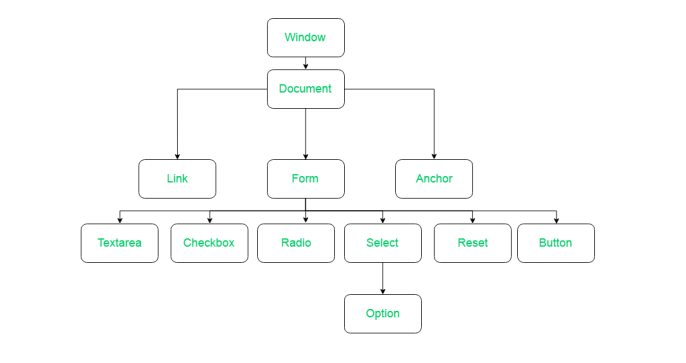
\includegraphics[width=1 \linewidth]{figure/dom}
	\end{center}
	\caption{Rappresentazione Document Object Model\label{fig:dom}}
\end{figure}
\subsection{Oggetti di dominio}
Come detto nel capitolo 4 la realizzazione è stata supportata dalla metolodologia agile, che ha portato ad avere più iterazioni riguardanti la fasi di analisi e l' ideazione degli oggetti di dominio che andranno a comporre il sistema. 
Di seguito in \textbf{\figurename~\ref{fig:primaIterazione}} è descritto in maniera molto semplificata il diagramma degli oggetti di dominio, risultato dall'analisi del progetto nella prima iterazione.\\
%%foto del diagramma della prima iterazione
\begin{figure}[!htb]
	\begin{center}
		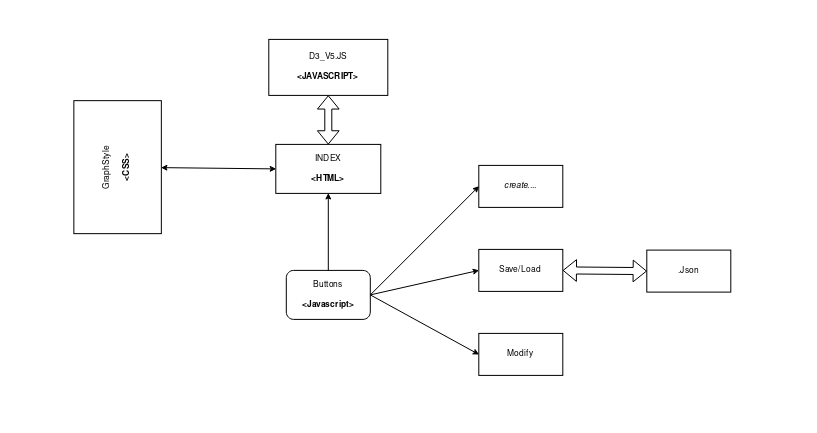
\includegraphics[width=1 \linewidth]{figure/primaIterazione}
	\end{center}
	\caption{Prima iterazione degli oggetti di dominio\label{fig:primaIterazione}}
\end{figure}
\newline
Come si nota la libreria D3.js è stata fin da subito pensata come punto centrale per le visualizzazioni. Per rendere la rappresentazione accessibile e utilizzabile in pieno si è scelto di realizzare tutte le primitive di interazione viste nel capitolo 5.\\
Una volta definite le interazioni i problemi che sono stati affrontati con maggior interesse per quanto concerne l'editor in esempio riguardano due importanti fattori che si ritrovano i qualunque software grafico: la facilità di impiego e l'ottenimento di una visualizzazione gradevole all'utente.
Durante una successiva analisi si è poi optato per alcune modifiche progettuali che sono mostrate nel diagramma ad oggetti di seguito in \figurename~\ref{fig:secondaIterazione} seguendo i principi espressi dal libro "UML distilled. Guida rapida al linguaggio di modellazione standard"\cite{UML:10}.\\
\begin{figure}[!htb]
	\begin{center}
		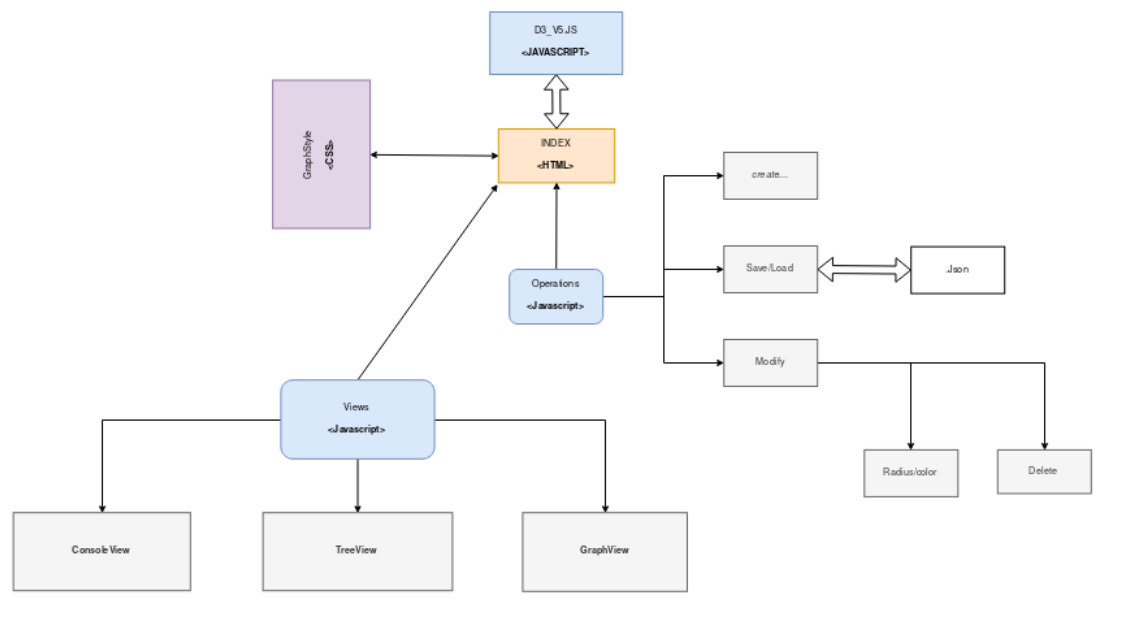
\includegraphics[width=1 \linewidth]{figure/secondaIterazione}
	\end{center}
	\caption{Seconda iterazione degli oggetti di dominio\label{fig:secondaIterazione}}
\end{figure}
Nell'ingegneria del software, \textbf{UML}, acronimo di Unified Modeling Language ovvero di "linguaggio di modellizzazione unificato" è un linguaggio di specifica basato sul paradigma orientato agli oggetti. Il nucleo del linguaggio fu definito nel 1996 da Grady Booch, Jim Rumbaugh e Ivar Jacobson. Lo stantard è tuttora gestito dall'Object Management Group. UML svolge un'importantissima funzione di "lingua franca" nella comunità della progettazione e programmazione ad oggetti utilizzato anche dalla gran parte della letteratura del settore informatico per descrivere soluzioni analitiche e progettuali in modo sintetico e comprensibile ad un vasto pubblico.
\subsection{Struttura dati}
Per quanto concerne la struttura dati su cui si basa la visualizzazione si è optato per una struttura ad oggetti ed in particolare si è scelto di utilizzare le strutture dello standard ECMAScript 6 quali Map e Set risultando essere una scelta migliore rispetto all'utilizzo di array per ragioni prestazionali, di sicurezza e di miglior accesso ai dati da rappresentare, spesso senza bisogno di iterare completamente su tutti i valori indicizzati al loro interno. Inoltre risultano essere oggetti specializzati: il \textbf{Set} garantisce l'unicità dei valori mentre l'oggetto Map conserva l'ordine di inserimento. Per completezza si ricorda inoltre che un oggetto \textbf{Map} contiene coppie $<KEY,VALUE>$ in cui qualunque valore, sia esso oggetto o tipo primitivo, può esser usato come chiave e come valore. Ad avvalorare la scelta si nota che entrambi sono oggetti \textit{iterable} quindi facili da iterare e hanno funzionamenti e prestazioni migliori in caso di frequenti aggiunte o rimozioni di valori.
Prima ancora di mostrare l'interfaccia e le modalità di impiego delle primitive analizzate nel capitolo 5 è necessario definire con chiarezza la struttura dati con cui l'utente andrà a lavorare ricordando infatti che una visualizzazione per buona che sia non ha valore senza la possibilità di analisi del dato di cui ne è la rappresentazione.
Come visto nel capitolo 3 un grafo clusterizzato $C$ è definito come una coppia $<G,T>$ in cui $G$ è l'underlying graph definito dalla coppia $<V,E>$ rispettivamente di nodi ed archi e $T$ è l'inclusion tree. Avendo chiaro questa definizione vi è la rappresentazione del grafo clusterizzato così come mostrato nella figura \figurename~\ref{fig:cgraphClass}.
\newpage
\begin{figure}[!htb]
	\begin{center}
		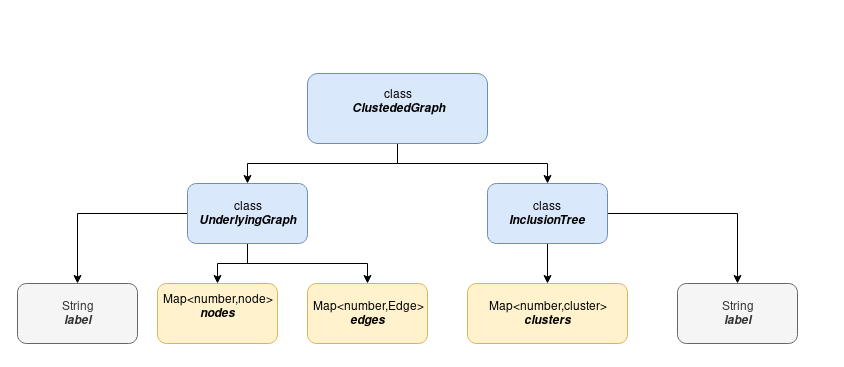
\includegraphics[width=1 \linewidth]{figure/cgraphClass}
	\end{center}
	\caption{Oggetto clusteredGraph\label{fig:cgraphClass}}
\end{figure}
Un \textit{clusteredGraph} è definito mediante un oggetto relativo all'underlying graph ed uno relativo all'inclusion tree.
Un \textit{UnderlyingGraph} è definito mediante una primitiva String che ne rappresenta l'etichetta e mediante due oggetti Map: Map<number,Node>, in cui sono elencati tutti i nodi di cui è composto il grafo e Map<number,Edge>, per gli archi appartenenti al grafo clusterizzato. 
Andando poi a ritroso nelle definizioni, nella figura \figurename~\ref{fig:nodeClass} è mostrato l'oggetto Nodo. Esso può essere definito mediante un costruttore di tre valori:
\begin{itemize}
	\item \textbf{label} di tipo primitivo String che ne definisce l'etichetta;
	\item \textbf{id} un numero, identificativo insieme alla sua etichetta ma ancor più personale, del nodo in questione;
	\item \textbf{rotationScheme} di tipo Set<number> in cui vengono salvati tutti gli ID degli archi che hanno quel nodo come nodo di partenza o di destinazione.
\end{itemize}
Ogni nodo è un elemento fondamentale dell'underlying graph da visualizzare e connettere.
\begin{figure}[!htb]
	\begin{center}
		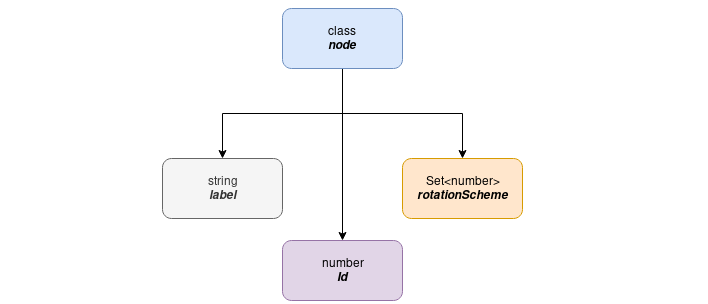
\includegraphics[width=1 \linewidth]{figure/nodeClass}
	\end{center}
	\caption{Oggetto nodo del underlying graph\label{fig:nodeClass}}
\end{figure}
Restando sempre nella creazione dell'oggetto \textit{UnderlyingGraph} del grafo clusterizzato risulta, esattamente come per l'oggetto \textit{node}, necessario fornire la definizione dell'oggetto relativo agli archi.
La classe dell'oggetto \textit{Edge} rappresentata in \figurename~\ref{fig:edgeClass} è definita mediante una stringa e tre valori numerici. La prima si riferisce all'etichetta dell'arco e non necessariamente dovrà essere unica, i valori numerici invece fanno riferimento all'id dell'arco al nodo sorgente e al nodo di fine arco. L'id risulta necessario non solo per unificare l'arco creato ma anche per essere inserito nel Set<number> \textit{rotationScheme} del nodo che lo vedrà collegato. Ogni arco collegherà poi un nodo di inizio fino ad un nodo di arrivo anche se non in maniera orientata, in quanto il nodo di inizio e il nodo di fine arco saranno solamente quelli relativi a dove l'utente vorrà che la visualizzazione dell'arco inizi e finisca. Per questo ogni elemento della classe arco avrà due valori numerici \textit{source} che conterrà l'id del nodo di partenza e \textit{target} con l'id del nodo di destinaione.
\newpage
\begin{figure}[!htb]
	\begin{center}
		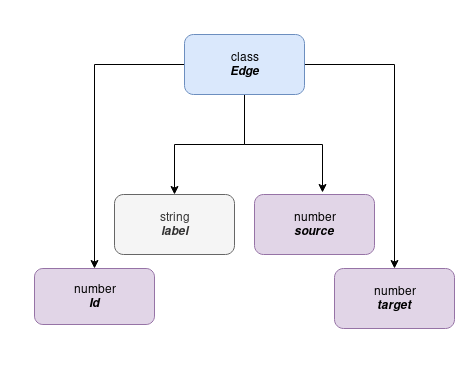
\includegraphics[width=1 \linewidth]{figure/edgeClass}
	\end{center}
	\caption{Oggetto arco dell'undelying graph\label{fig:edgeClass}}
\end{figure}

Termina la definizione della classe \textit{UnderlyingGraph} si può passare a quella della classe \textit{InclusionTree}. Ogni oggetto appartenente a questa classe possiede una etichetta definita come tipo String, esattamente come per la sua controparte grafo, e una lista contenente i cluster che fanno parte dell'albero di inclusione, di tipo Map<number,Cluster>.
Andando a ritroso anche in questa struttura si vuol definire di seguito la classe \textit{Cluster}.
Un oggetto \textit{cluster} come mostrato nella figura \figurename~\ref{fig:clusterClass} è definito mediante un costruttore con cinque attributi di seguito riportati:
\begin{itemize}
	\item \textbf{label} di tipo String che ne rappresenta l'etichetta;
	\item \textbf{level} di tipo number, definisce il livello ovvero la profondità a cui il cluster si troverà all'interno dell'albero di inclusione;
	\item \textbf{cildren} di tipo Set<number> e che contiene gli id dei cluster di profondità superiore collegati con il cluster di interesse, ovvero i suoi figli;
	\item \textbf{parents} di tipo Set<number> contenente gli id dei cluster di profondità inferiore e che sono collegati al cluster di interesse, ovvero i suoi genitori;
	\item \textbf{nodes} di tipo Set<number> contenente gli id dei nodi che sono contenuti all'interno del cluster
\end{itemize}

\begin{figure}[!htb]
	\begin{center}
		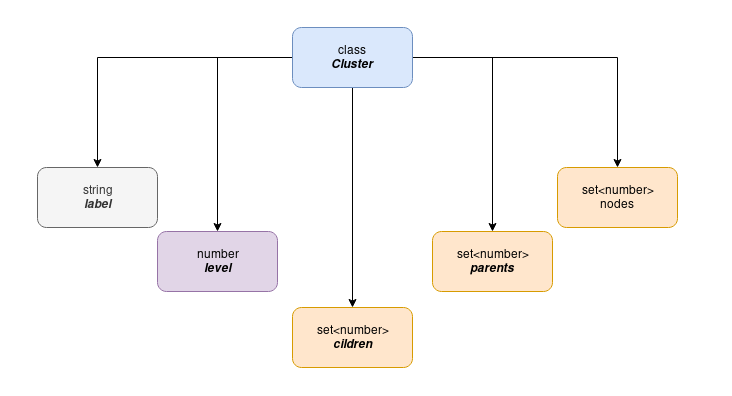
\includegraphics[width=1 \linewidth]{figure/clusterClass}
	\end{center}
	\caption{Oggetto cluster dell'inclusion Tree\label{fig:clusterClass}}
\end{figure}
\section{Log-in ed interfacce}
	\subsection{Inizializzazione}
Al momento del log-in iniziale l'utente si troverà la schermata mostrata nella \figurename~\ref{fig:interfaccia}. Come è possibile notare da subito sono stati utilizzati molti dei principi di visualizzazione visti in precedenza cominciando dall'impiego e della posizione dei bottoni necessari per le interazioni dell'utente. È stato lasciando inoltre grande spazio per quanto concerne il piano di lavoro principale che, come si vedrà successivamente, rimarrà inalterato anche cambiando l'interfaccia utilizzata. Anche l'impiego di colori caldi come il blu rispetto al piano di lavoro di colore chiaro lascia intendere la maggiore importanza ed evidenza che deve avere il secondo rispetto al resto dell'interfaccia. Ogni qualvolta l'utente vorrà interagire con il sistema sarà sufficiente cliccare una delle operazioni, che saranno viste nel capitolo successivo, per poter avere una risposta.
\begin{figure}[!htb]
	\begin{center}
		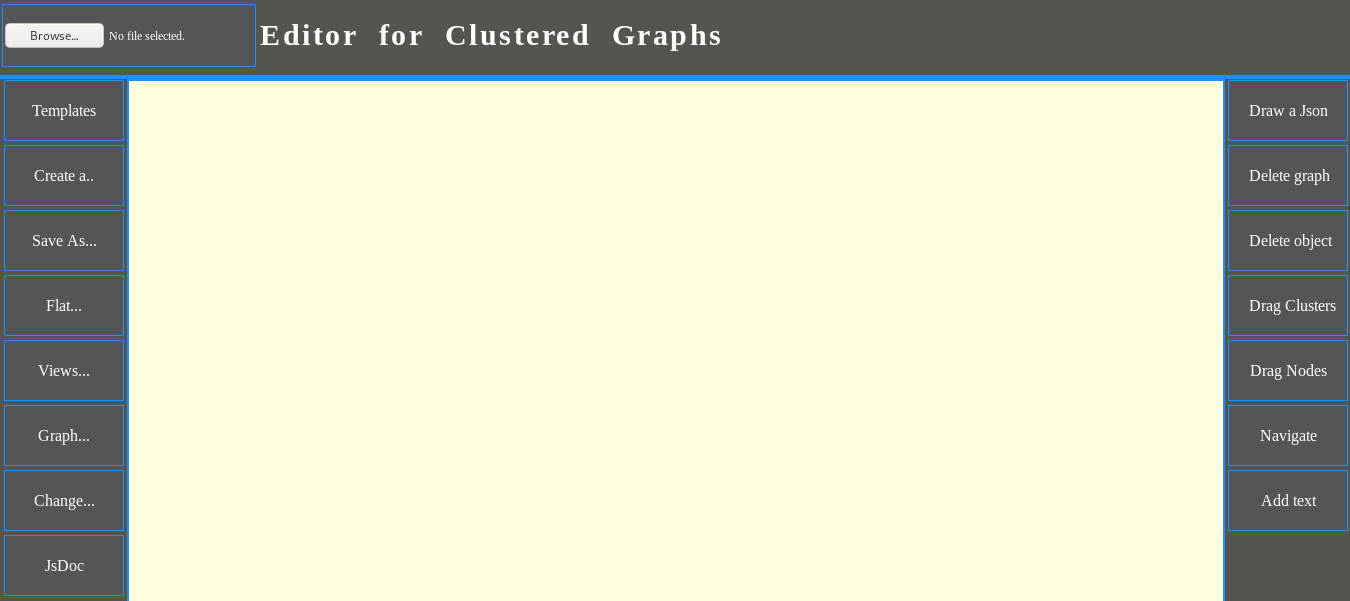
\includegraphics[width=1 \linewidth]{figure/interfaccia}
	\end{center}
	\caption{Log-in nel sistema\label{fig:interfaccia}}
\end{figure}
Come definito nel capitolo relativo alle primitive, è necessario poter dare all'utente la possibilità di eseguire un encoding dei dati. Per questo ogni qualvolta verrà richiesto al sistema di eseguire il log-in iniziale oppure un encode della visualizzazione il sistema risponderà con una inizializzazione. Durante la prima inzializzazione in cui sarà creata la classe \textit{clusteredGraph} e tutto ciò che ne comprende, sarà generato l'svg \#cgraph su cui si basa il piano di lavoro e con cui l'utente andrà ad interagire ed analizzare. Tutte le operazioni e le visualizzazioni saranno eseguite proprio su questo svg creato con l'ausilio della libreria grafica\textbf{ D3.js}.\\
Generato l'svg principale, sempre durante l'inizializzazione del log-in, verrà collegato ad altri tre oggetti svg di seguito elencati e che lo compongono:
\begin{itemize}
	\item \textbf{\#c\_cluster} che andrà a rappresentare la visualizzazione di tutti i cluster; 
	\item \textbf{\#c\_node} ovvero l'svg che rappresenta l'insieme dei nodi da visualizzare;
	\item \textbf{\#c\_edge} che rappresenterà gli archi che collegano i nodi dell'underlying graph.
\end{itemize}
La divisione degli svg che andranno a comporre quello relativo al piano di lavoro è necessaria per molteplici fattori, primo fra tutti il fatto che poter scindere una entità monolitica in molteplici oggetti è uno dei traguardi dello sviluppo software. Inoltre è possibile in questo modo poter trattare, come sarà analizzato meglio in seguito, le tre entità che rappresentano la classe \textit{ClusteredGraph} come oggetti a se stanti.\\
Una volta che l'utente ha avuto accesso al sistema ed è stato introdotto il concetto di svg e di piano di lavoro, è possibile cominciare a definire quello di interfacce e dei diversi piani di lavoro.
Essendo basato su una coppia $<G,T>$ che compongono il grafo clusterizzato $C$ si è deciso di implementare la funzione di encode dando all'utente la possibilità di scelta tra due viste separate riportate nelle sezioni seguenti. Prima di passare all'analisi di queste rappresentazioni è bene anticipare la struttura dell'algoritmo, mostrato nella \figurename~\ref{fig:viewAlg}, che il sistema andrà ad eseguire ogni volta l'utente chiederà mediante una interazione l'operazione di encode dei dati. Ad ogni richiesta sopra descritta il sistema confronterà la vista su cui attualmente l'utente lavora con quella richiesta ritornando nel caso in cui le due viste siano uguali ed eliminando la vista visualizzata e creano quella richiesta nel caso contrario.\\
La strategia scelta dell'eliminare e ricreare un oggetto si sposa bene con i principi per la visualizzazione visti in precedenza. In questo modo l'utente andrà ad interfacciarsi con una unica visualizzazione alla volta ed il piano di lavoro resterà libero evitando ogni volta di dimezzare la grandezza dello stesso per far posto a visualizzazioni che non sono funzionali alle trasformazioni ma che hanno esclusivamente scopi di analisi.
\begin{figure}[!htb]
	\begin{center}
		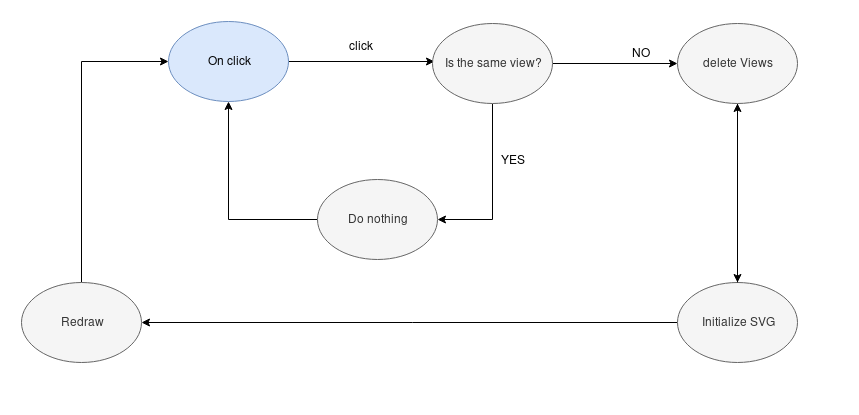
\includegraphics[width=1 \linewidth]{figure/viewAlg}
	\end{center}
	\caption{Struttura dell'algoritmo dell'operazione di encode\label{fig:viewAlg}}
\end{figure}

\subsection{Graph-view}
La visualizzazione a grafo, anche definita graph-view è la visualizzazione di default ed è anche quella con cui l'utente si interfaccerà maggiormente. La graph-view è infatti l'unica vista con cui l'utente può avere una interazione di grado tre, ovvero il grado massimo, in cui può interagire sulle modifiche e le trasformazioni non solo riguardo la visualizzazione ma anche sui dati.\\
\begin{figure}[!htb]
	\begin{center}
		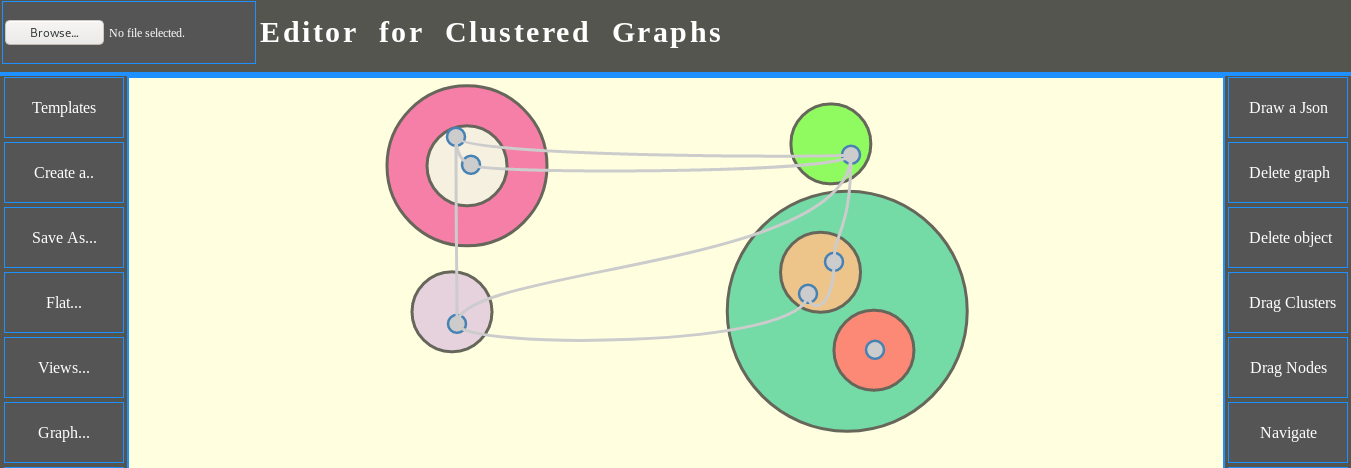
\includegraphics[width=1 \linewidth]{figure/graphView}
	\end{center}
	\caption{Graph View\label{fig:graphView}}
\end{figure}
\newline
Come si può notare dalla \figurename~\ref{fig:graphView} il modello di visualizzazione riprende quello Node-link in cui i "Node" sono differenziati in due elementi, rappresentando non solo i nodi del grafo ma anche i cluster dell'albero di inclusione. La differenza tra queste due entità a livello di visualizzazione può essere vista mediante due diversi fattori: il colore ed il raggio.
Per quanto riguarda il colore dei nodi risulta essere fisso in quanto ogni nodo rappresenterà sempre lo stesso elemento che cambierà per quanto riguarda la posizione o il cluster di appartenenza ma non nella visualizzazione. Anche il raggio del nodo, che verrà definito $r_n$, ha un valore fisso non dipendente da nessuna variabile.
Per quanto riguarda i cluster invece il colore, che di default presenta una casualità nella propria visualizzazione, varia per ogni cluster definendo una ulteriore variabile che ne definisce l'unicità.
Il raggio dei cluster definito $r_c$, al contrario di quello dei nodi che come abbiamo visto è fisso esso è dipendente da variabili come visto nel capitolo 5.

\subsection{Tree-view}
Non avendo un limite al numero di nodi e di cluster visualizzabili la graph view può portare ad una eccessivo disordine dato dalla quantità. L'occhio umano vede una rappresentazione organizzata in maniera notevolmente migliore rispetto ad una piatta e priva di profondità. Per questo l'utente in qualunque momento durante una sessione di lavoro potrà interagire con il sistema e passare da una visualizzazione a grafo ad una dell'inclusion tree in cui però saranno rappresentati anche i nodi e gli archi dell'underlying graph ovvero ad una visualizzazione ad albero.\\
Ogni volta che si chiederà questa operazione, il sistema risponderà eliminando la visualizzazione e inizializzandone una nuova con un encode sugli stessi dati rappresentati in precedenza. Questa visualizzazione sarà un svg detto \#\_ctree che possiederà grandezza uguale a quella dell' \#cgraph ma senza una divisione degli elementi che andranno a comporre la rappresentazione, come era invece necessario per la visualizzazione a grafo.\\
Questa rappresentazione risulterà comunque essere un modello node-link ma, al contrario che nella graph view, in cui non si avrà necessità di inserire forze per una visualizzazione ottimale essendo una semplice rappresentazione "layered" con l'aggiunta di archi che collegano le foglie tra loro. Nella \figurename~\ref{fig:treeView} è mostrato lo stesso grafo visualizzato in precedenza nella graph-view e visto nella figura \figurename~\ref{fig:graphView}.
Nella visualizzazione ad albero il raggio dei cluster e dei nodi risulta essere la stesso anche se ciò che caratterizza una foglia, che sia essa un cluster vuoto oppure un nodo all'interno di un cluster, è il diverso colore diverso rispetto ai nodi interni.
Essendo un sistema in cui non vi è una soglia massima del numero di nodi è di cluster definibili o importabili si possono presentare situazioni limite. Per questo sono state implementate due diverse tipologie di tree-view, entrambe discendenti: ad albero verticale ed orizzontale.
All'utente è lasciata la scelta di quale delle due utilizzare. È consigliabile ai fini di una buona visualizzazione l'utilizzo di una rappresentazione verticale nel caso in cui si hanno tanti cluster sullo stesso livello ma la profondità dell'albero sia relativamente bassa mentre è preferibile utilizzare una visualizzazione ad albero orizzontale, con la radice centrale a sinistra dell'svg, nel caso in cui si hanno pochi cluster per ogni livello ma si abbia una profondità maggiore da gestire.
\begin{figure}[!htb]
	\begin{center}
		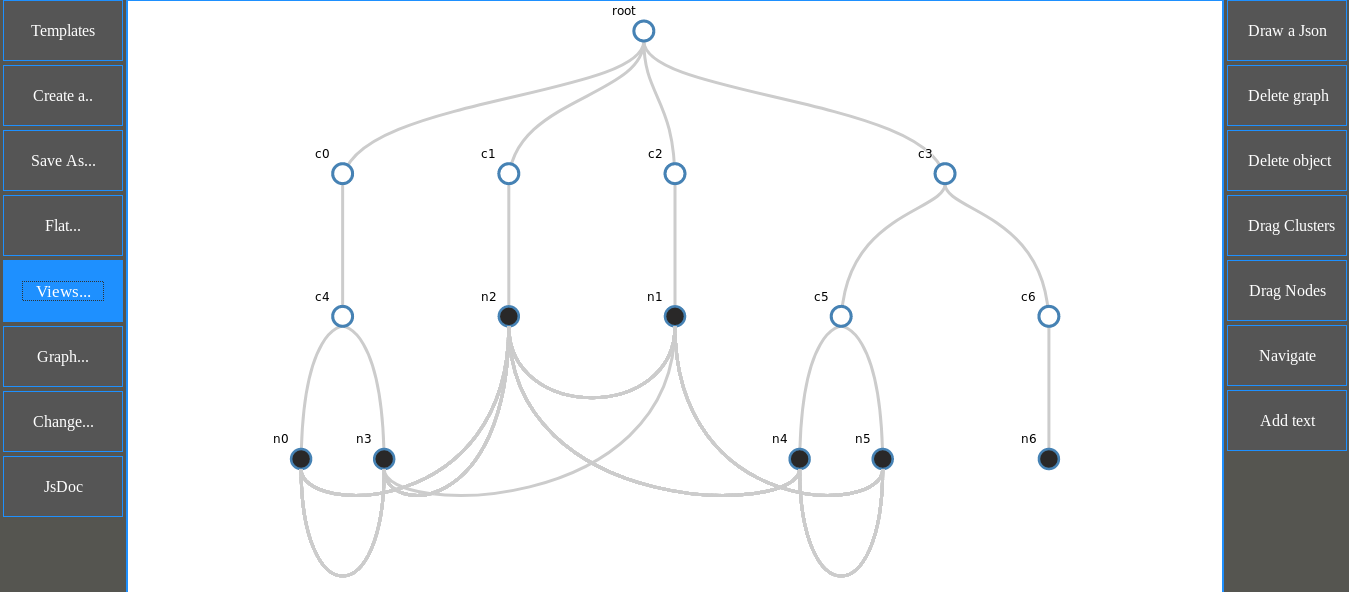
\includegraphics[width=1 \linewidth]{figure/treeView}
	\end{center}
	\caption{tree View\label{fig:treeView}}
\end{figure}
	\subsection{Console-view}
Oltre all'operazione di encode vista si ha la necessità di dover mostrare, sotto richiesta dell'utente, dei log riguardanti i cambiamenti eseguiti durante una stessa sessione di lavoro. Per questo è stata introdotta una terza vista definita \textit{console-view} che risolve questa problematica.
Mediante una interazione similare a quelle viste in precedenza, l'utente può accedere a questa visualizzazione. Il sistema risponderà eliminando il precedente svg che sia esso \#cgraph oppure \#ctree e creerà un nuovo svg di dimensioni uguali ed in cui saranno inseriti i messaggi lasciati all'utente delle ultime $n$ operazioni eseguite. Ogni operazione infatti, nel momento in cui viene richiesta dall'utente, mentre viene eseguita salva un valore di tipo String all'interno di un oggetto Map<number,String> \textit{logs} inzializzato al log-in all'inizio della sessione di lavoro dell'utente.
La vista sarà similare a quella mostrata nella \figurename~\ref{fig:consoleView}, nella quale oltre al messaggio che ricorda l'operazione richiesta ed eseguita, sarà visualizzato l'orario in cui l'utente ha interagito con il sistema. Terminate le viste e delucidato il lettore sulle operazioni di encode eseguibili si passa adesso a definire con più chiarezza le operazioni di filtraggio
\begin{figure}[!htb]
	\begin{center}
		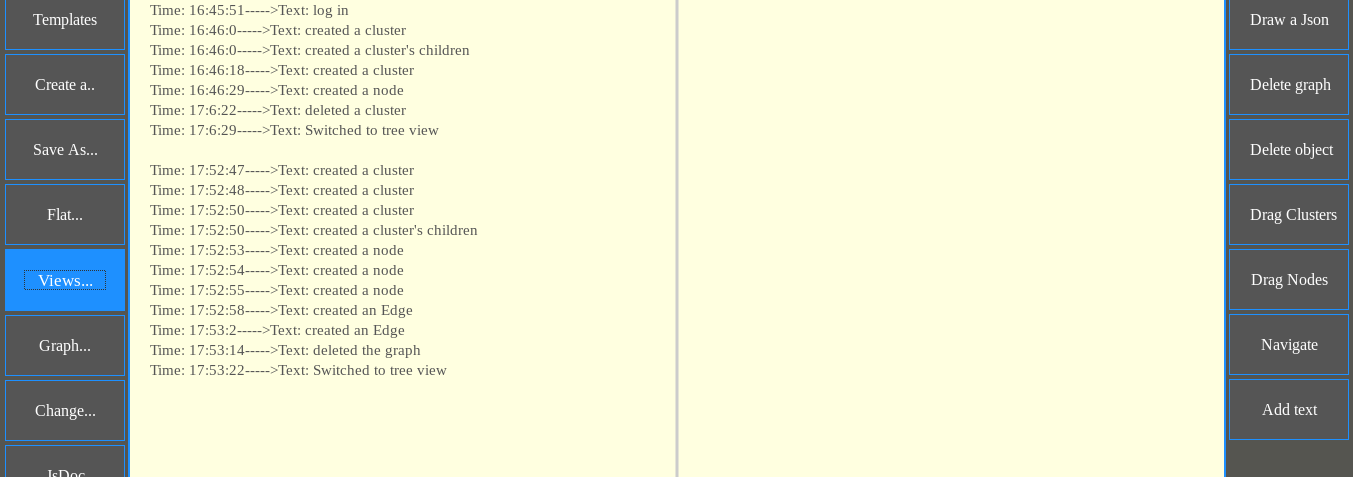
\includegraphics[width=1 \linewidth]{figure/consoleView}
	\end{center}
	\caption{Graph View\label{fig:consoleView}}
\end{figure}
\newpage
\subsection{Filtraggio degli oggetti}
Una operazione di filtraggio permette di mostrare un sottoinsieme di dati secondo certe regole, ovvero ciò che può esser definito come uno zoom semantico. Si immagini un grafo clusterizzato di dimensioni notevoli o comunque con una delle classi di oggetti che lo compongono che, in un momento particolare, abbia un rilievo maggiore rispetto agli altri. Volendo lavorare solamente su un particolare oggetto è possibile stando nella \textit{graph-view} eseguire una operazione di filtraggio su una delle tre componenti come mostrato nella \figurename~\ref{fig:clustersOnly} che fa riferimento  alla \figurename~\ref{fig:graphView} in cui però l'utente ha necessità di vedere solamente la disposizione dei cluster nel dettaglio.
\begin{figure}[!htb]
	\begin{center}
		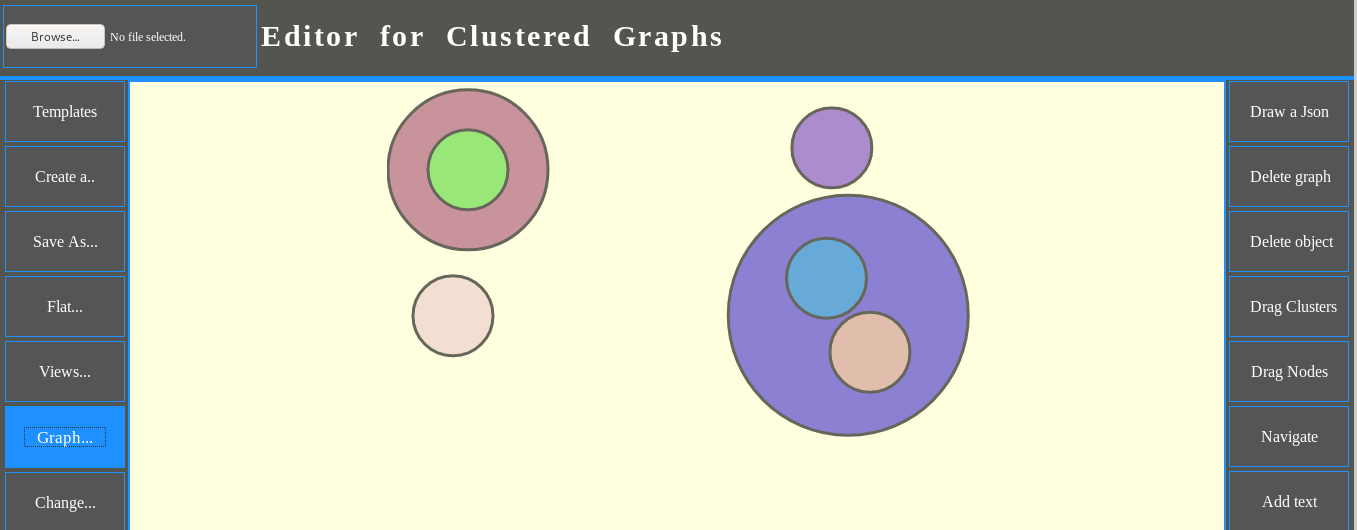
\includegraphics[width=1 \linewidth]{figure/clustersOnly}
	\end{center}
	\caption{visualizzazione dei soli cluster\label{fig:clustersOnly}}
\end{figure}
Essendo un grafo clusterizzato un grafo planare, per quanto riguarda gli archi si ha la necessità che essi non intersechino nulla ad di fuori del loro nodo \textit{source} e del nodo \textit{target}. In un grafo di grandi dimensioni o comunque con un numero relativamente alto di archi questa esigenza sarebbe di difficile analisi. Per questo facendo riferimento alla \figurename~\ref{fig:graphView} l'utente può avere accesso ad una rappresentazione filtrata sugli archi come mostrato in \figurename~\ref{fig:edgesOnly}. Partendo dalla visualizzazione \textit{graph-view}, filtrando una particolare classe tra le sue componenti, si avrà un maggiore dettaglio per quell'oggetto, ma si perderanno due gradi di integrazione, passando dalla possibilità di interazione che permette la trasformazione della visualizzazione e dei dati, a una integrazione di grado $0$ che consentirà solo l'analisi, anche se è sempre possibile tornare alla rappresentazione di default per poter continuare la sessione di lavoro.  
\begin{figure}[!htb]
	\begin{center}
		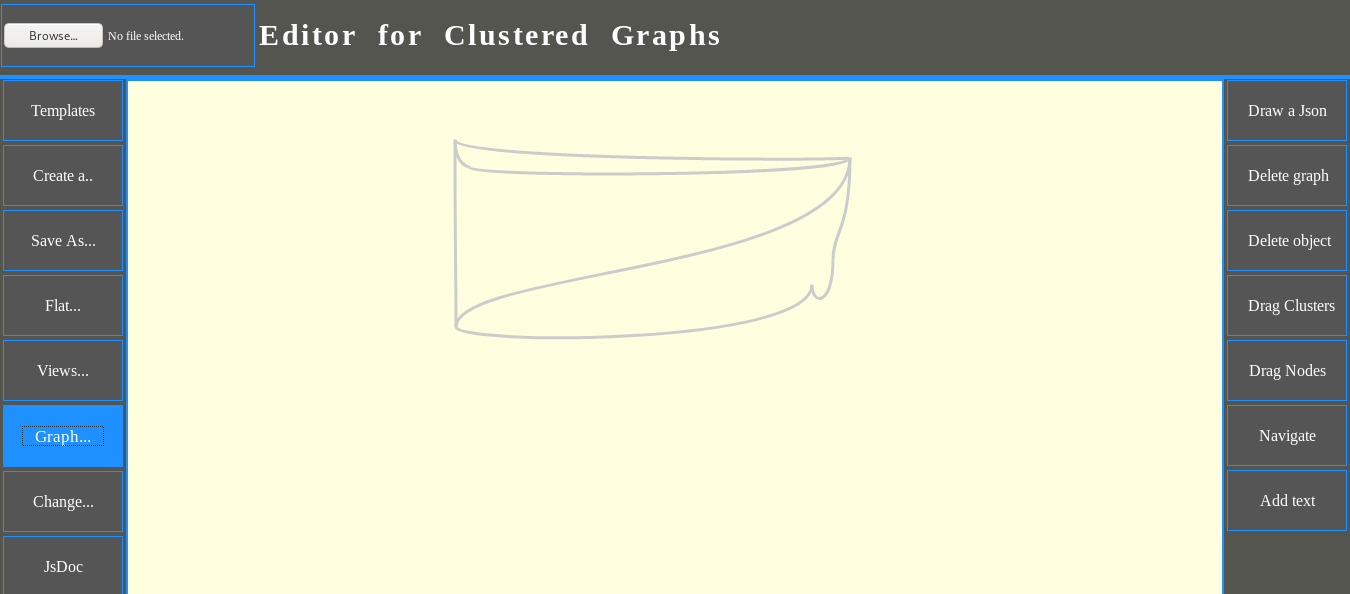
\includegraphics[width=1 \linewidth]{figure/edgesOnly}
	\end{center}
	\caption{Visualizzazione dei soli archi\label{fig:edgesOnly}}
\end{figure}
}